\documentclass[aspectratio=169,11pt]{beamer}
% =====================================================================
%  pds-beamer.tex — Estilo común de las transparencias.
%
%  Uso (desde teoría/Tx/transparencias/):
%     \documentclass[aspectratio=169,11pt]{beamer}
%     % =====================================================================
%  pds-beamer.tex — Estilo común de las transparencias.
%
%  Uso (desde teoría/Tx/transparencias/):
%     \documentclass[aspectratio=169,11pt]{beamer}
%     % =====================================================================
%  pds-beamer.tex — Estilo común de las transparencias.
%
%  Uso (desde teoría/Tx/transparencias/):
%     \documentclass[aspectratio=169,11pt]{beamer}
%     \input{../../comun/pds-beamer}
%     \title{...}  \subtitle{Tema x · ...}
%     \begin{document}
%       \portada
%       ...
%     \end{document}
%  Compilar con:  latexmk -xelatex  (o «make» desde teoría/)
% =====================================================================

\usetheme{Boadilla}
\usecolortheme{orchid}
\usefonttheme{professionalfonts}
\setbeamercovered{transparent}
\setbeamersize{text margin left=0.8cm, text margin right=0.8cm}
\setbeamertemplate{navigation symbols}{}
\setbeamertemplate{itemize item}[square]
\setbeamertemplate{itemize subitem}[circle]
\setbeamertemplate{itemize subsubitem}[triangle]
\setbeamertemplate{enumerate item}[square]
\setbeamertemplate{enumerate subitem}[circle]
\setbeamertemplate{caption}{\raggedright\insertcaption\par}

\input{../../comun/pds-comun.tex}

% Tipografía: Fira Sans + Fira Math (legibles en proyector)
\usepackage{fontspec}
\usepackage{unicode-math}
% Se cargan por nombre de fichero para que funcionen con cualquier
% instalación de TeX Live (o MiKTeX) sin instalar fuentes en el sistema.
\setmainfont{FiraSans}[Extension=.otf, UprightFont=*-Regular, BoldFont=*-SemiBold,
  ItalicFont=*-Italic, BoldItalicFont=*-SemiBoldItalic]
\setsansfont{FiraSans}[Extension=.otf, UprightFont=*-Regular, BoldFont=*-SemiBold,
  ItalicFont=*-Italic, BoldItalicFont=*-SemiBoldItalic]
\setmonofont{FiraMono}[Extension=.otf, UprightFont=*-Regular, BoldFont=*-Medium, AutoFakeSlant=0.15, Scale=0.92]
\setmathfont{FiraMath-Regular.otf}
\setmathfont{latinmodern-math.otf}[range={"229B,"22EE,"22F1}]

% Colores del tema ajustados a la paleta común (más contraste)
\setbeamercolor{structure}{fg=pdsazul}
\setbeamercolor{alerted text}{fg=pdsrojo}
\setbeamercolor{example text}{fg=pdsverde}
\setbeamercolor{block title}{bg=pdsazul, fg=white}
\setbeamercolor{block body}{bg=pdsfondo}
\setbeamercolor{block title alerted}{bg=pdsrojo, fg=white}
\setbeamercolor{block body alerted}{bg=pdsrojo!6}
\setbeamercolor{block title example}{bg=pdsverde, fg=white}
\setbeamercolor{block body example}{bg=pdsverde!6}
\setbeamercolor{frametitle}{fg=pdsazul, bg=white}
\setbeamerfont{frametitle}{size=\large, series=\bfseries}
\setbeamerfont{block title}{size=\normalsize, series=\bfseries}
\setbeamertemplate{blocks}[rounded][shadow=false]

% Logo en la esquina superior derecha de cada transparencia
\pgfdeclareimage[height=0.8cm]{logo}{../../comun/ucm.png}
\addtobeamertemplate{frametitle}{}{%
  \begin{tikzpicture}[remember picture, overlay]
    \node[anchor=north east, inner sep=0pt] at ([xshift=-0.25cm, yshift=-0.2cm]current page.north east) {\pgfuseimage{logo}};
  \end{tikzpicture}}

% Datos de portada
\author[\autorescorto]{\autores}
\institute[UCM]{\footnotesize\departamento\\\universidad}
\date[\curso]{\footnotesize\grado\\\curso}

\newcommand{\portada}{%
  \begin{frame}[plain]
    \begin{center}
      
\includegraphics[height=1.9cm]{../../comun/ucm.png}
    \end{center}
    \vspace{-0.4cm}
    \titlepage
  \end{frame}}

% Índice al empezar cada sección
\AtBeginSection[]{%
  \begin{frame}{Contenido}
    \tableofcontents[currentsection, hideothersubsections]
  \end{frame}}

\renewcommand{\pdscodesize}{\scriptsize}

% Utilidades
% \herramienta{T1-convolucion-continua}: enlace a la página publicada de
% herramientas/html (se abre en el navegador, sin instalar nada).
% \herramientaservidor{server/....py}: app que necesita Python (bokeh serve).
\newcommand{\urlherramientas}{https://ucm-237.github.io/PdS/}
\newcommand{\herramienta}[1]{%
  \par\vfill\hfill{\scriptsize\color{pdsgris}\faIcon\ \href{\urlherramientas#1.html}{Herramienta interactiva: \texttt{#1}}}}
\newcommand{\herramientaservidor}[1]{%
  \par\vfill\hfill{\scriptsize\color{pdsgris}\faIcon\ Herramienta interactiva (con Python): \texttt{herramientas/#1}}}
\newcommand{\faIcon}{\textbf{▶}}
\newcommand{\gris}[1]{{\color{pdsgris}#1}}
\newcommand{\nota}[1]{\par\vspace{2pt}{\footnotesize\color{pdsgris}\textit{#1}}\par}
% Nota sobre una errata de versiones anteriores (solo con \ERRATAS)
\newcommand{\errata}[1]{\iferratas\nota{Errata de versiones anteriores: #1}\fi}
\newcommand{\apuntes}[1]{\nota{Más detalle en los apuntes, #1.}}

% Bloques con nombre en castellano
\newenvironment{definicion}[1][Definición]{\begin{block}{#1}}{\end{block}}
\newenvironment{importante}[1][Importante]{\begin{alertblock}{#1}}{\end{alertblock}}
\newenvironment{ejemplo}[1][Ejemplo]{\begin{exampleblock}{#1}}{\end{exampleblock}}

%     \title{...}  \subtitle{Tema x · ...}
%     \begin{document}
%       \portada
%       ...
%     \end{document}
%  Compilar con:  latexmk -xelatex  (o «make» desde teoría/)
% =====================================================================

\usetheme{Boadilla}
\usecolortheme{orchid}
\usefonttheme{professionalfonts}
\setbeamercovered{transparent}
\setbeamersize{text margin left=0.8cm, text margin right=0.8cm}
\setbeamertemplate{navigation symbols}{}
\setbeamertemplate{itemize item}[square]
\setbeamertemplate{itemize subitem}[circle]
\setbeamertemplate{itemize subsubitem}[triangle]
\setbeamertemplate{enumerate item}[square]
\setbeamertemplate{enumerate subitem}[circle]
\setbeamertemplate{caption}{\raggedright\insertcaption\par}

% =====================================================================
%  pds-comun.tex — Paquetes, colores y estilos de código comunes a
%  transparencias, apuntes y hojas de ejercicios. Compilar con XeLaTeX.
%  No cargar directamente: lo cargan pds-beamer.tex y pds-apuntes.tex.
% =====================================================================

\usepackage{polyglossia}
\setmainlanguage{spanish}
\usepackage{mathtools}
\usepackage{graphicx}
\usepackage{booktabs}
\usepackage{multirow}
\usepackage{array}
\usepackage{xcolor}
\usepackage{tikz}
\usetikzlibrary{positioning,arrows.meta,calc,shapes.geometric,decorations.pathreplacing}
\usepackage{listings}
\usepackage{siunitx}
\sisetup{output-decimal-marker={,}, group-separator={\,}, per-mode=symbol}

% Notas de erratas de versiones anteriores: no se imprimen salvo que se
% defina \ERRATAS antes de cargar el estilo (make ERRATAS=1)
\newif\iferratas
\ifdefined\ERRATAS \erratastrue \fi

% Ruta común (logo y figuras compartidas)
\providecommand{\rutacomun}{../../comun/}
\input{\rutacomun datos.tex}

% ---------------------------------------------------------------------
%  Paleta (la misma que usan las figuras generadas con Python,
%  ver comun/pds_estilo.py)
% ---------------------------------------------------------------------
\definecolor{pdsazul}{HTML}{2B3A8C}
\definecolor{pdsrojo}{HTML}{C0392B}
\definecolor{pdsverde}{HTML}{1E7B4F}
\definecolor{pdsnaranja}{HTML}{D9822B}
\definecolor{pdsgris}{HTML}{5A5A66}
\definecolor{pdsfondo}{HTML}{F3F4FA}
\definecolor{pdscodigo}{HTML}{F7F7F2}

% ---------------------------------------------------------------------
%  Diagramas de bloques (TikZ)
% ---------------------------------------------------------------------
\tikzset{
  bloque/.style={rectangle, rounded corners=2pt, draw=pdsazul!80, fill=pdsfondo,
                 very thick, minimum height=8mm, minimum width=14mm, align=center},
  sumador/.style={circle, draw=pdsazul!80, fill=pdsfondo, thick, inner sep=1.5pt},
  flecha/.style={-{Stealth[length=2.2mm]}, thick, pdsgris},
}

% ---------------------------------------------------------------------
%  Código: Python y Matlab en paralelo
% ---------------------------------------------------------------------
\newcommand{\pdscodesize}{\footnotesize}
\lstdefinestyle{pds}{
  basicstyle=\ttfamily\pdscodesize,
  keywordstyle=\color{pdsazul}\bfseries,
  commentstyle=\color{pdsverde}\itshape,
  stringstyle=\color{pdsrojo},
  numbers=none,
  backgroundcolor=\color{pdscodigo},
  frame=single, rulecolor=\color{pdsgris!40}, framerule=0.4pt,
  xleftmargin=2pt, xrightmargin=2pt, aboveskip=2pt, belowskip=2pt,
  columns=fullflexible, keepspaces=true,
  showstringspaces=false, breaklines=true, tabsize=4,
  upquote=true,
  % Con XeLaTeX, listings desordena los caracteres no ASCII junto a
  % dígitos («2π» sale «π2»): se sustituyen por su versión matemática.
  literate={π}{{$\pi$}}1 {δ}{{$\delta$}}1 {ω}{{$\omega$}}1 {Ω}{{$\Omega$}}1
           {≈}{{$\approx$}}1 {µ}{{$\mu$}}1 {·}{{$\cdot$}}1 {α}{{$\alpha$}}1
           {á}{{á}}1 {é}{{é}}1 {í}{{í}}1 {ó}{{ó}}1 {ú}{{ú}}1 {ñ}{{ñ}}1 {¿}{{¿}}1,
}
\lstdefinestyle{python}{style=pds, language=Python,
  morekeywords={as,True,False,None}}
\lstdefinestyle{matlab}{style=pds, language=Matlab,
  morekeywords={function,end,true,false}}

% \codigo{<ruta sin extensión>} muestra el mismo ejemplo en Python
% y en Matlab, uno al lado del otro. Los ficheros viven en
% ../codigo/python/<nombre>.py y ../codigo/matlab/<nombre>.m y se
% ejecutan en las pruebas (make prueba-codigo).
\newcommand{\rutacodigo}{../codigo/}
\newcommand{\codigoetiqueta}[1]{{\sffamily\scriptsize\bfseries\color{pdsgris}#1}}
\newcommand{\codigo}[2][]{%
  \par\noindent
  \begin{minipage}[t]{0.495\linewidth}
    \codigoetiqueta{Python}\par\vspace{1pt}
    \lstinputlisting[style=python,#1]{\rutacodigo python/#2.py}
  \end{minipage}\hfill
  \begin{minipage}[t]{0.495\linewidth}
    \codigoetiqueta{Matlab}\par\vspace{1pt}
    \lstinputlisting[style=matlab,#1]{\rutacodigo matlab/#2.m}
  \end{minipage}\par}

\input{\rutacomun notacion.tex}


% Tipografía: Fira Sans + Fira Math (legibles en proyector)
\usepackage{fontspec}
\usepackage{unicode-math}
% Se cargan por nombre de fichero para que funcionen con cualquier
% instalación de TeX Live (o MiKTeX) sin instalar fuentes en el sistema.
\setmainfont{FiraSans}[Extension=.otf, UprightFont=*-Regular, BoldFont=*-SemiBold,
  ItalicFont=*-Italic, BoldItalicFont=*-SemiBoldItalic]
\setsansfont{FiraSans}[Extension=.otf, UprightFont=*-Regular, BoldFont=*-SemiBold,
  ItalicFont=*-Italic, BoldItalicFont=*-SemiBoldItalic]
\setmonofont{FiraMono}[Extension=.otf, UprightFont=*-Regular, BoldFont=*-Medium, AutoFakeSlant=0.15, Scale=0.92]
\setmathfont{FiraMath-Regular.otf}
\setmathfont{latinmodern-math.otf}[range={"229B,"22EE,"22F1}]

% Colores del tema ajustados a la paleta común (más contraste)
\setbeamercolor{structure}{fg=pdsazul}
\setbeamercolor{alerted text}{fg=pdsrojo}
\setbeamercolor{example text}{fg=pdsverde}
\setbeamercolor{block title}{bg=pdsazul, fg=white}
\setbeamercolor{block body}{bg=pdsfondo}
\setbeamercolor{block title alerted}{bg=pdsrojo, fg=white}
\setbeamercolor{block body alerted}{bg=pdsrojo!6}
\setbeamercolor{block title example}{bg=pdsverde, fg=white}
\setbeamercolor{block body example}{bg=pdsverde!6}
\setbeamercolor{frametitle}{fg=pdsazul, bg=white}
\setbeamerfont{frametitle}{size=\large, series=\bfseries}
\setbeamerfont{block title}{size=\normalsize, series=\bfseries}
\setbeamertemplate{blocks}[rounded][shadow=false]

% Logo en la esquina superior derecha de cada transparencia
\pgfdeclareimage[height=0.8cm]{logo}{../../comun/ucm.png}
\addtobeamertemplate{frametitle}{}{%
  \begin{tikzpicture}[remember picture, overlay]
    \node[anchor=north east, inner sep=0pt] at ([xshift=-0.25cm, yshift=-0.2cm]current page.north east) {\pgfuseimage{logo}};
  \end{tikzpicture}}

% Datos de portada
\author[\autorescorto]{\autores}
\institute[UCM]{\footnotesize\departamento\\\universidad}
\date[\curso]{\footnotesize\grado\\\curso}

\newcommand{\portada}{%
  \begin{frame}[plain]
    \begin{center}
      
\includegraphics[height=1.9cm]{../../comun/ucm.png}
    \end{center}
    \vspace{-0.4cm}
    \titlepage
  \end{frame}}

% Índice al empezar cada sección
\AtBeginSection[]{%
  \begin{frame}{Contenido}
    \tableofcontents[currentsection, hideothersubsections]
  \end{frame}}

\renewcommand{\pdscodesize}{\scriptsize}

% Utilidades
% \herramienta{T1-convolucion-continua}: enlace a la página publicada de
% herramientas/html (se abre en el navegador, sin instalar nada).
% \herramientaservidor{server/....py}: app que necesita Python (bokeh serve).
\newcommand{\urlherramientas}{https://ucm-237.github.io/PdS/}
\newcommand{\herramienta}[1]{%
  \par\vfill\hfill{\scriptsize\color{pdsgris}\faIcon\ \href{\urlherramientas#1.html}{Herramienta interactiva: \texttt{#1}}}}
\newcommand{\herramientaservidor}[1]{%
  \par\vfill\hfill{\scriptsize\color{pdsgris}\faIcon\ Herramienta interactiva (con Python): \texttt{herramientas/#1}}}
\newcommand{\faIcon}{\textbf{▶}}
\newcommand{\gris}[1]{{\color{pdsgris}#1}}
\newcommand{\nota}[1]{\par\vspace{2pt}{\footnotesize\color{pdsgris}\textit{#1}}\par}
% Nota sobre una errata de versiones anteriores (solo con \ERRATAS)
\newcommand{\errata}[1]{\iferratas\nota{Errata de versiones anteriores: #1}\fi}
\newcommand{\apuntes}[1]{\nota{Más detalle en los apuntes, #1.}}

% Bloques con nombre en castellano
\newenvironment{definicion}[1][Definición]{\begin{block}{#1}}{\end{block}}
\newenvironment{importante}[1][Importante]{\begin{alertblock}{#1}}{\end{alertblock}}
\newenvironment{ejemplo}[1][Ejemplo]{\begin{exampleblock}{#1}}{\end{exampleblock}}

%     \title{...}  \subtitle{Tema x · ...}
%     \begin{document}
%       \portada
%       ...
%     \end{document}
%  Compilar con:  latexmk -xelatex  (o «make» desde teoría/)
% =====================================================================

\usetheme{Boadilla}
\usecolortheme{orchid}
\usefonttheme{professionalfonts}
\setbeamercovered{transparent}
\setbeamersize{text margin left=0.8cm, text margin right=0.8cm}
\setbeamertemplate{navigation symbols}{}
\setbeamertemplate{itemize item}[square]
\setbeamertemplate{itemize subitem}[circle]
\setbeamertemplate{itemize subsubitem}[triangle]
\setbeamertemplate{enumerate item}[square]
\setbeamertemplate{enumerate subitem}[circle]
\setbeamertemplate{caption}{\raggedright\insertcaption\par}

% =====================================================================
%  pds-comun.tex — Paquetes, colores y estilos de código comunes a
%  transparencias, apuntes y hojas de ejercicios. Compilar con XeLaTeX.
%  No cargar directamente: lo cargan pds-beamer.tex y pds-apuntes.tex.
% =====================================================================

\usepackage{polyglossia}
\setmainlanguage{spanish}
\usepackage{mathtools}
\usepackage{graphicx}
\usepackage{booktabs}
\usepackage{multirow}
\usepackage{array}
\usepackage{xcolor}
\usepackage{tikz}
\usetikzlibrary{positioning,arrows.meta,calc,shapes.geometric,decorations.pathreplacing}
\usepackage{listings}
\usepackage{siunitx}
\sisetup{output-decimal-marker={,}, group-separator={\,}, per-mode=symbol}

% Notas de erratas de versiones anteriores: no se imprimen salvo que se
% defina \ERRATAS antes de cargar el estilo (make ERRATAS=1)
\newif\iferratas
\ifdefined\ERRATAS \erratastrue \fi

% Ruta común (logo y figuras compartidas)
\providecommand{\rutacomun}{../../comun/}
\input{\rutacomun datos.tex}

% ---------------------------------------------------------------------
%  Paleta (la misma que usan las figuras generadas con Python,
%  ver comun/pds_estilo.py)
% ---------------------------------------------------------------------
\definecolor{pdsazul}{HTML}{2B3A8C}
\definecolor{pdsrojo}{HTML}{C0392B}
\definecolor{pdsverde}{HTML}{1E7B4F}
\definecolor{pdsnaranja}{HTML}{D9822B}
\definecolor{pdsgris}{HTML}{5A5A66}
\definecolor{pdsfondo}{HTML}{F3F4FA}
\definecolor{pdscodigo}{HTML}{F7F7F2}

% ---------------------------------------------------------------------
%  Diagramas de bloques (TikZ)
% ---------------------------------------------------------------------
\tikzset{
  bloque/.style={rectangle, rounded corners=2pt, draw=pdsazul!80, fill=pdsfondo,
                 very thick, minimum height=8mm, minimum width=14mm, align=center},
  sumador/.style={circle, draw=pdsazul!80, fill=pdsfondo, thick, inner sep=1.5pt},
  flecha/.style={-{Stealth[length=2.2mm]}, thick, pdsgris},
}

% ---------------------------------------------------------------------
%  Código: Python y Matlab en paralelo
% ---------------------------------------------------------------------
\newcommand{\pdscodesize}{\footnotesize}
\lstdefinestyle{pds}{
  basicstyle=\ttfamily\pdscodesize,
  keywordstyle=\color{pdsazul}\bfseries,
  commentstyle=\color{pdsverde}\itshape,
  stringstyle=\color{pdsrojo},
  numbers=none,
  backgroundcolor=\color{pdscodigo},
  frame=single, rulecolor=\color{pdsgris!40}, framerule=0.4pt,
  xleftmargin=2pt, xrightmargin=2pt, aboveskip=2pt, belowskip=2pt,
  columns=fullflexible, keepspaces=true,
  showstringspaces=false, breaklines=true, tabsize=4,
  upquote=true,
  % Con XeLaTeX, listings desordena los caracteres no ASCII junto a
  % dígitos («2π» sale «π2»): se sustituyen por su versión matemática.
  literate={π}{{$\pi$}}1 {δ}{{$\delta$}}1 {ω}{{$\omega$}}1 {Ω}{{$\Omega$}}1
           {≈}{{$\approx$}}1 {µ}{{$\mu$}}1 {·}{{$\cdot$}}1 {α}{{$\alpha$}}1
           {á}{{á}}1 {é}{{é}}1 {í}{{í}}1 {ó}{{ó}}1 {ú}{{ú}}1 {ñ}{{ñ}}1 {¿}{{¿}}1,
}
\lstdefinestyle{python}{style=pds, language=Python,
  morekeywords={as,True,False,None}}
\lstdefinestyle{matlab}{style=pds, language=Matlab,
  morekeywords={function,end,true,false}}

% \codigo{<ruta sin extensión>} muestra el mismo ejemplo en Python
% y en Matlab, uno al lado del otro. Los ficheros viven en
% ../codigo/python/<nombre>.py y ../codigo/matlab/<nombre>.m y se
% ejecutan en las pruebas (make prueba-codigo).
\newcommand{\rutacodigo}{../codigo/}
\newcommand{\codigoetiqueta}[1]{{\sffamily\scriptsize\bfseries\color{pdsgris}#1}}
\newcommand{\codigo}[2][]{%
  \par\noindent
  \begin{minipage}[t]{0.495\linewidth}
    \codigoetiqueta{Python}\par\vspace{1pt}
    \lstinputlisting[style=python,#1]{\rutacodigo python/#2.py}
  \end{minipage}\hfill
  \begin{minipage}[t]{0.495\linewidth}
    \codigoetiqueta{Matlab}\par\vspace{1pt}
    \lstinputlisting[style=matlab,#1]{\rutacodigo matlab/#2.m}
  \end{minipage}\par}

\input{\rutacomun notacion.tex}


% Tipografía: Fira Sans + Fira Math (legibles en proyector)
\usepackage{fontspec}
\usepackage{unicode-math}
% Se cargan por nombre de fichero para que funcionen con cualquier
% instalación de TeX Live (o MiKTeX) sin instalar fuentes en el sistema.
\setmainfont{FiraSans}[Extension=.otf, UprightFont=*-Regular, BoldFont=*-SemiBold,
  ItalicFont=*-Italic, BoldItalicFont=*-SemiBoldItalic]
\setsansfont{FiraSans}[Extension=.otf, UprightFont=*-Regular, BoldFont=*-SemiBold,
  ItalicFont=*-Italic, BoldItalicFont=*-SemiBoldItalic]
\setmonofont{FiraMono}[Extension=.otf, UprightFont=*-Regular, BoldFont=*-Medium, AutoFakeSlant=0.15, Scale=0.92]
\setmathfont{FiraMath-Regular.otf}
\setmathfont{latinmodern-math.otf}[range={"229B,"22EE,"22F1}]

% Colores del tema ajustados a la paleta común (más contraste)
\setbeamercolor{structure}{fg=pdsazul}
\setbeamercolor{alerted text}{fg=pdsrojo}
\setbeamercolor{example text}{fg=pdsverde}
\setbeamercolor{block title}{bg=pdsazul, fg=white}
\setbeamercolor{block body}{bg=pdsfondo}
\setbeamercolor{block title alerted}{bg=pdsrojo, fg=white}
\setbeamercolor{block body alerted}{bg=pdsrojo!6}
\setbeamercolor{block title example}{bg=pdsverde, fg=white}
\setbeamercolor{block body example}{bg=pdsverde!6}
\setbeamercolor{frametitle}{fg=pdsazul, bg=white}
\setbeamerfont{frametitle}{size=\large, series=\bfseries}
\setbeamerfont{block title}{size=\normalsize, series=\bfseries}
\setbeamertemplate{blocks}[rounded][shadow=false]

% Logo en la esquina superior derecha de cada transparencia
\pgfdeclareimage[height=0.8cm]{logo}{../../comun/ucm.png}
\addtobeamertemplate{frametitle}{}{%
  \begin{tikzpicture}[remember picture, overlay]
    \node[anchor=north east, inner sep=0pt] at ([xshift=-0.25cm, yshift=-0.2cm]current page.north east) {\pgfuseimage{logo}};
  \end{tikzpicture}}

% Datos de portada
\author[\autorescorto]{\autores}
\institute[UCM]{\footnotesize\departamento\\\universidad}
\date[\curso]{\footnotesize\grado\\\curso}

\newcommand{\portada}{%
  \begin{frame}[plain]
    \begin{center}
      
\includegraphics[height=1.9cm]{../../comun/ucm.png}
    \end{center}
    \vspace{-0.4cm}
    \titlepage
  \end{frame}}

% Índice al empezar cada sección
\AtBeginSection[]{%
  \begin{frame}{Contenido}
    \tableofcontents[currentsection, hideothersubsections]
  \end{frame}}

\renewcommand{\pdscodesize}{\scriptsize}

% Utilidades
% \herramienta{T1-convolucion-continua}: enlace a la página publicada de
% herramientas/html (se abre en el navegador, sin instalar nada).
% \herramientaservidor{server/....py}: app que necesita Python (bokeh serve).
\newcommand{\urlherramientas}{https://ucm-237.github.io/PdS/}
\newcommand{\herramienta}[1]{%
  \par\vfill\hfill{\scriptsize\color{pdsgris}\faIcon\ \href{\urlherramientas#1.html}{Herramienta interactiva: \texttt{#1}}}}
\newcommand{\herramientaservidor}[1]{%
  \par\vfill\hfill{\scriptsize\color{pdsgris}\faIcon\ Herramienta interactiva (con Python): \texttt{herramientas/#1}}}
\newcommand{\faIcon}{\textbf{▶}}
\newcommand{\gris}[1]{{\color{pdsgris}#1}}
\newcommand{\nota}[1]{\par\vspace{2pt}{\footnotesize\color{pdsgris}\textit{#1}}\par}
% Nota sobre una errata de versiones anteriores (solo con \ERRATAS)
\newcommand{\errata}[1]{\iferratas\nota{Errata de versiones anteriores: #1}\fi}
\newcommand{\apuntes}[1]{\nota{Más detalle en los apuntes, #1.}}

% Bloques con nombre en castellano
\newenvironment{definicion}[1][Definición]{\begin{block}{#1}}{\end{block}}
\newenvironment{importante}[1][Importante]{\begin{alertblock}{#1}}{\end{alertblock}}
\newenvironment{ejemplo}[1][Ejemplo]{\begin{exampleblock}{#1}}{\end{exampleblock}}

\graphicspath{{../figuras/}}

\title[T4 · Filtros IIR]{Filtros}
\subtitle{Tema 4 · Parte 3: diseño de filtros IIR}

\begin{document}
\portada

% =====================================================================
\section{De $s$ a $z$}

\begin{frame}{Diseño IIR a partir de un filtro continuo}
  \begin{itemize}
    \item El diseño de filtros continuos está resuelto (parte 2). Se aprovecha: se diseña $H_a(s)$ y se convierte en $H(z)$.
    \item La conversión debe conservar lo esencial:
    \begin{itemize}
      \item el eje $j\omega$ debe ir a la circunferencia unidad, para que la respuesta en frecuencia se conserve;
      \item el semiplano izquierdo debe ir al interior del círculo, para que un $H_a$ estable dé un $H$ estable;
      \item $H(z)$ debe ser racional, para implementarlo con una ecuación en diferencias.
    \end{itemize}
    \item Dos métodos:
    \begin{itemize}
      \item \alert{Invarianza al impulso}: $h[n]$ son muestras de $h_a(t)$.
      \item \alert{Transformada bilineal}: sustitución algebraica de $s$ por una función de $z$.
    \end{itemize}
  \end{itemize}
\end{frame}

\begin{frame}{Invarianza al impulso}
  \begin{columns}[T]
    \begin{column}{0.5\textwidth}
      \footnotesize
      Se muestrea la respuesta al impulso: $h[n]=T\,h_a(nT)$.
      \begin{itemize}
        \item Con fracciones simples:
        \[
          H_a(s)=\sum_k\frac{r_k}{s-p_k}\ \to\ H(z)=\sum_k\frac{T\,r_k}{1-\e^{p_kT}z^{-1}}
        \]
        \item Cada polo $p_k$ pasa a $\e^{p_kT}$: si $\Re p_k<0$, $\abs{\e^{p_kT}}<1$. Estable.
        \item La respuesta en frecuencia es la del Tema 2:
        \[
          H(\e^{j\Omega})=\sum_{m}H_a\Big(j\frac{\Omega-2\pi m}{T}\Big)
        \]
        con \alert{aliasing} si $H_a$ no está limitado a $\abs{\omega}<\pi/T$.
      \end{itemize}
    \end{column}
    \begin{column}{0.48\textwidth}
      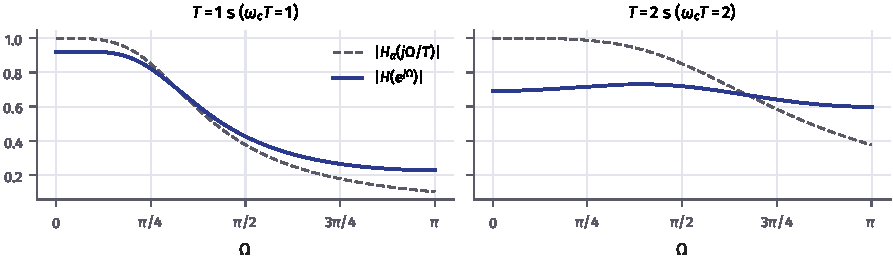
\includegraphics[width=\linewidth]{invarianza}
      \footnotesize
      \begin{itemize}
        \item Butterworth de orden 2 con $\omega_c=1$\,rad/s. Con $T=2$\,s el solapamiento es enorme.
        \item Solo sirve para paso bajo y paso banda; nunca para paso alto ni supresor.
      \end{itemize}
    \end{column}
  \end{columns}
\end{frame}

\begin{frame}{Transformada bilineal}
  \begin{columns}[T]
    \begin{column}{0.5\textwidth}
      \small
      \[
        s=\frac2T\,\frac{1-z^{-1}}{1+z^{-1}}\qquad\Longleftrightarrow\qquad z=\frac{1+sT/2}{1-sT/2}
      \]
      \begin{itemize}
        \item Sale de integrar con la regla del trapecio: $y[n]=y[n-1]+\frac T2(x[n]+x[n-1])$ $\Rightarrow$ $\frac1s\approx\frac T2\frac{1+z^{-1}}{1-z^{-1}}$.
        \item El semiplano izquierdo va al \alert{interior} del círculo y el eje $j\omega$ \alert{sobre} la circunferencia. Sin aliasing.
        \item En $s=j\omega$, $z=\e^{j\Omega}$:
        \[
          j\omega=\frac2T\,\frac{\e^{j\Omega/2}-\e^{-j\Omega/2}}{\e^{j\Omega/2}+\e^{-j\Omega/2}}=j\frac2T\tan\frac\Omega2
        \]
      \end{itemize}
    \end{column}
    \begin{column}{0.48\textwidth}
      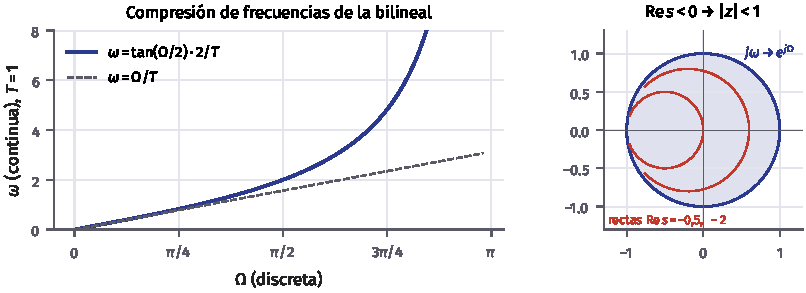
\includegraphics[width=\linewidth]{bilineal}
      \begin{importante}[Compresión de frecuencias]
        \small $\omega=\frac2T\tan\frac\Omega2$: todo el eje $[0,\infty)$ cabe en $[0,\pi)$. Las frecuencias se deforman, pero los niveles (rizados, atenuaciones) se conservan.
      \end{importante}
    \end{column}
  \end{columns}
\end{frame}

\begin{frame}{Predistorsión de frecuencias}
  \small
  \begin{itemize}
    \item Para que el filtro discreto tenga sus bordes en $\Omega_p$ y $\Omega_s$, el continuo debe tenerlos en
    \[
      \omega_p=\frac2T\tan\frac{\Omega_p}{2},\qquad\omega_s=\frac2T\tan\frac{\Omega_s}{2}.
    \]
    \item $T$ no tiene por qué ser el periodo de muestreo: se cancela entre la predistorsión y la bilineal. Se suele tomar \alert{$T=2$}: $\omega=\tan(\Omega/2)$ y $s=\frac{1-z^{-1}}{1+z^{-1}}$.
    \item Los ceros en el infinito de un paso bajo continuo aparecen en $z=-1$ ($\Omega=\pi$).
  \end{itemize}
  \begin{importante}[Procedimiento]
    \begin{enumerate}\setlength{\itemsep}{0pt}
      \item Especificaciones discretas: $\Omega=2\pi f/f_s$ para cada borde; $\alpha_p$ y $\alpha_s$ no cambian.
      \item Predistorsión: $\omega=\tan(\Omega/2)$.
      \item Diseño del filtro continuo (prototipo y transformación si no es paso bajo).
      \item Bilineal: $H(z)=H_a\big(\frac{1-z^{-1}}{1+z^{-1}}\big)$ (\texttt{bilinear} con $f_s=1/T=0{,}5$).
    \end{enumerate}
  \end{importante}
\end{frame}

% =====================================================================
\section{Ejemplos}

\begin{frame}{Ejemplo: paso bajo de Butterworth}
  \begin{ejemplo}[Enunciado]
    $f_s=200$\,kHz; banda de paso hasta 25\,kHz con rizado máximo de 0,5\,dB; atenuación mínima de 15\,dB desde 55\,kHz.
  \end{ejemplo}
  \begin{columns}[T]
    \begin{column}{0.5\textwidth}
      \small
      \begin{align*}
        &\Omega_p=2\pi\tfrac{25}{200}=0{,}25\pi,\quad\Omega_s=0{,}55\pi\\
        &\omega_p=\tan(0{,}125\pi)=0{,}4142,\quad\omega_s=1{,}1708\\
        &N\ge\frac{\log_{10}(30{,}62/0{,}1220)}{2\log_{10}(1{,}1708/0{,}4142)}=2{,}66\to3\\
        &\omega_c\in[0{,}588,\ 0{,}663]
      \end{align*}
    \end{column}
    \begin{column}{0.48\textwidth}
      \small
      Con $\omega_c=0{,}588$ y la bilineal:
      \[
        H(z)=\frac{0{,}0662\,(1+z^{-1})^3}{1-0{,}9357z^{-1}+0{,}5672z^{-2}-0{,}1016z^{-3}}
      \]
      \gris{Tres ceros en $z=-1$, como se esperaba.}
    \end{column}
  \end{columns}
\end{frame}

\begin{frame}{Ejemplo: respuesta del filtro}
  \begin{center}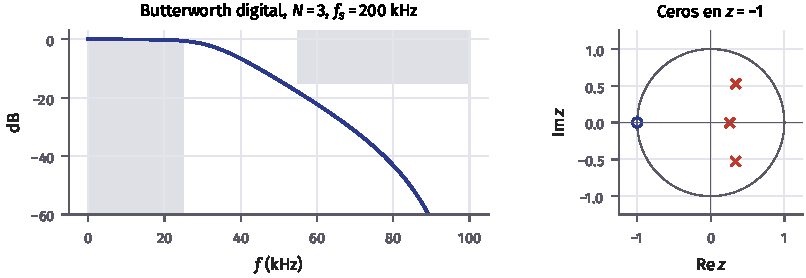
\includegraphics[width=0.9\linewidth]{iir_paso_bajo}\end{center}
  \nota{Cumple con margen la banda de supresión: a 55\,kHz atenúa 18\,dB. Las tres raíces de $(1+z^{-1})^3$ anulan la respuesta en $\Omega=\pi$ ($f=100$\,kHz).}
\end{frame}

\begin{frame}{En código: predistorsión y bilineal}
  \codigo[basicstyle=\ttfamily\fontsize{6.2}{7.2}\selectfont]{iir_bilineal}
\end{frame}

\begin{frame}{Diseño directo con Matlab y \texttt{scipy.signal}}
  \begin{itemize}
    \item Las funciones de orden y diseño hacen la predistorsión y la bilineal si se omite \texttt{'s'} (o \texttt{analog=True}) y las frecuencias se dan \alert{normalizadas a Nyquist}, $\Omega/\pi\in[0,1]$.
    \item En \texttt{scipy.signal} también se pueden dar en hercios con el argumento \texttt{fs}.
  \end{itemize}
  \footnotesize
  \renewcommand{\arraystretch}{1.2}
  \begin{center}
    \begin{tabular}{@{}lll@{}}
      \toprule
      & Matlab / Octave & Python (\texttt{scipy.signal})\\\midrule
      Orden & \texttt{[N,Wn]=buttord(Wp,Ws,Rp,Rs)} & \texttt{N,Wn=buttord(Wp,Ws,Rp,Rs)}\\
      Diseño & \texttt{[b,a]=butter(N,Wn,'high')} & \texttt{b,a=butter(N,Wn,'highpass')}\\
      Paso banda & \texttt{Wn=[W1 W2]}, tipo por defecto & \texttt{Wn=[W1,W2]}, \texttt{'bandpass'}\\
      Supresor & \texttt{'stop'} & \texttt{'bandstop'}\\
      Secciones de orden 2 & \texttt{[z,p,k]=butter(...); zp2sos} & \texttt{butter(..., output='sos')}\\
      Respuesta & \texttt{freqz(b,a)} & \texttt{freqz(b,a)}, \texttt{sosfreqz(sos)}\\
      Filtrado & \texttt{filter(b,a,x)}, \texttt{sosfilt} & \texttt{lfilter(b,a,x)}, \texttt{sosfilt(sos,x)}\\\bottomrule
    \end{tabular}
  \end{center}
  \nota{Igual con \texttt{cheb1ord}/\texttt{cheby1}, \texttt{cheb2ord}/\texttt{cheby2} y \texttt{ellipord}/\texttt{ellip}.}
\end{frame}

\begin{frame}{Ejemplos: paso alto y paso banda}
  \begin{center}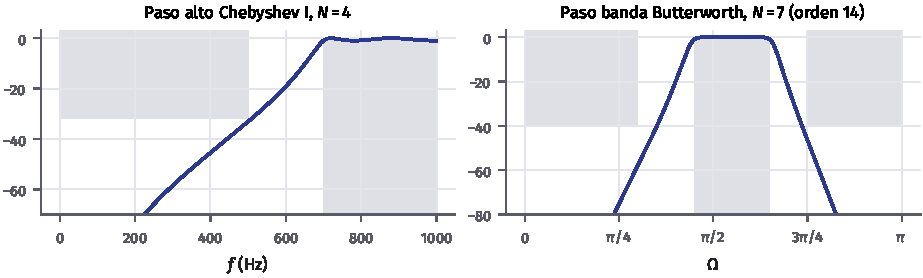
\includegraphics[height=0.4\textheight]{iir_ejemplos}\end{center}
  \footnotesize
  \begin{columns}[T]
    \begin{column}{0.5\textwidth}
      \alert{Chebyshev I paso alto}, $f_s=2$\,kHz: paso desde 700\,Hz (1\,dB), supresión por debajo de 500\,Hz (32\,dB).
      $\Omega_p=0{,}7\pi\to\hat\omega_p=1{,}9626$; $\Omega_s=0{,}5\pi\to\hat\omega_s=1$. Prototipo: $\omega_s=\hat\omega_p/\hat\omega_s=1{,}9626$,
      $N\ge\frac{\mathrm{arccosh}(78{,}2)}{\mathrm{arccosh}(1{,}9626)}=3{,}90\to4$.
    \end{column}
    \begin{column}{0.5\textwidth}
      \alert{Butterworth paso banda}: paso en $[0{,}45\pi,0{,}65\pi]$ (1\,dB), supresión fuera de $[0{,}3\pi,0{,}75\pi]$ (40\,dB).
      $\hat\omega$: 0,8541; 1,6319; 0,5095; 2,4142. $\hat\omega_0^2=1{,}3937$, $B=0{,}7778$,
      $\omega_s=\min(2{,}86;\ 2{,}36)=2{,}36$, $N\ge6{,}14\to7$ (orden 14).
    \end{column}
  \end{columns}
\end{frame}

\begin{frame}{En código: paso banda en secciones de orden 2}
  \codigo[basicstyle=\ttfamily\fontsize{6.8}{7.8}\selectfont]{iir_paso_banda}
  \nota{En forma directa, un IIR de orden alto es muy sensible al redondeo de los coeficientes: se implementa como cascada de secciones de orden 2.}
\end{frame}

% =====================================================================
\section{Otras herramientas}

\begin{frame}{Transformaciones de frecuencia en discreto}
  \small
  También se puede diseñar un paso bajo discreto $H_{\text{LP}}(z)$ con corte $\Omega_c$ y transformarlo sustituyendo $z^{-1}$ por un filtro paso todo $G(\hat z^{-1})$, que lleva la circunferencia unidad sobre sí misma:
  \renewcommand{\arraystretch}{1.7}
  \begin{center}
    \begin{tabular}{@{}lll@{}}
      \toprule
      Destino & $z^{-1}\to$ & Parámetro\\\midrule
      Paso bajo ($\hat\Omega_c$) & $\dfrac{\hat z^{-1}-\alpha}{1-\alpha\hat z^{-1}}$ & $\alpha=\dfrac{\sin\big((\Omega_c-\hat\Omega_c)/2\big)}{\sin\big((\Omega_c+\hat\Omega_c)/2\big)}$\\
      Paso alto ($\hat\Omega_c$) & $-\dfrac{\hat z^{-1}+\alpha}{1+\alpha\hat z^{-1}}$ & $\alpha=-\dfrac{\cos\big((\Omega_c+\hat\Omega_c)/2\big)}{\cos\big((\Omega_c-\hat\Omega_c)/2\big)}$\\\bottomrule
    \end{tabular}
  \end{center}
  \begin{itemize}\footnotesize
    \item Hay transformaciones análogas de orden 2 a paso banda y supresor (Oppenheim y Schafer, capítulo 7).
    \item Con $\Omega_c=\hat\Omega_c=\pi/2$, el paso alto es $\alpha=0$: $z\to-z$, que invierte el espectro ($h[n]\to(-1)^nh[n]$).
  \end{itemize}
\end{frame}

\begin{frame}{Invarianza al impulso y bilineal}
  \footnotesize
  \renewcommand{\arraystretch}{1.25}
  \begin{center}
    \begin{tabular}{@{}p{0.22\textwidth}p{0.34\textwidth}p{0.34\textwidth}@{}}
      \toprule
      & Invarianza al impulso & Bilineal\\\midrule
      Relación & $z=\e^{sT}$ (para los polos) & $s=\frac2T\frac{1-z^{-1}}{1+z^{-1}}$\\
      Frecuencias & Lineal: $\Omega=\omega T$ & Comprimidas: $\omega=\frac2T\tan\frac\Omega2$\\
      Aliasing & Sí & No\\
      Tipos de filtro & Paso bajo y paso banda & Todos\\
      Conserva & La forma de $h(t)$ & Los niveles de $\abs{H}$ (rizados, atenuaciones)\\
      Uso & Modelar un sistema continuo, cuando importa $h(t)$ & Diseño de filtros selectivos\\\bottomrule
    \end{tabular}
  \end{center}
  \herramienta{server/T4\_Filtros\_IIR\_Discretizacion.py}
\end{frame}

% =====================================================================
\section*{Resumen}
\begin{frame}{Conceptos importantes}
  \begin{columns}[T]
    \begin{column}{0.5\textwidth}
      \begin{itemize}
        \item IIR $=$ filtro continuo $+$ conversión $s\to z$.
        \item Invarianza al impulso: $h[n]=Th_a(nT)$, polos $\e^{p_kT}$, aliasing.
        \item Bilineal: $s=\frac{1-z^{-1}}{1+z^{-1}}$ ($T=2$), sin aliasing, para todos los tipos.
      \end{itemize}
    \end{column}
    \begin{column}{0.5\textwidth}
      \begin{itemize}
        \item Predistorsión: $\omega=\tan(\Omega/2)$ en cada borde.
        \item Matlab/\texttt{scipy}: frecuencias normalizadas a Nyquist y sin \texttt{'s'}.
        \item Órdenes altos: secciones de orden 2.
      \end{itemize}
    \end{column}
  \end{columns}
  \bigskip
  \gris{Apuntes del Tema 4, sección 3 · Hoja de ejercicios, ejercicios 8–11.}
\end{frame}

\end{document}
